\documentclass[tikz,border=8pt]{standalone}
\usepackage[T1]{fontenc}
\usepackage{tikz}
\usetikzlibrary{arrows.meta,positioning}
\definecolor{blue}{RGB}{32,94,180}
\definecolor{green}{RGB}{43,150,136}
\definecolor{purple}{RGB}{105,98,178}
\definecolor{gold}{RGB}{190,132,45}
\definecolor{textgray}{RGB}{38,45,56}
\tikzset{
  step/.style={draw=#1, fill=#1!8, rounded corners=3pt, thick, align=center,
    minimum width=29mm, minimum height=11mm, text=textgray, font=\sffamily\small},
  arrow/.style={-{Latex[length=2.2mm]}, thick, draw=textgray!70}
}
\begin{document}
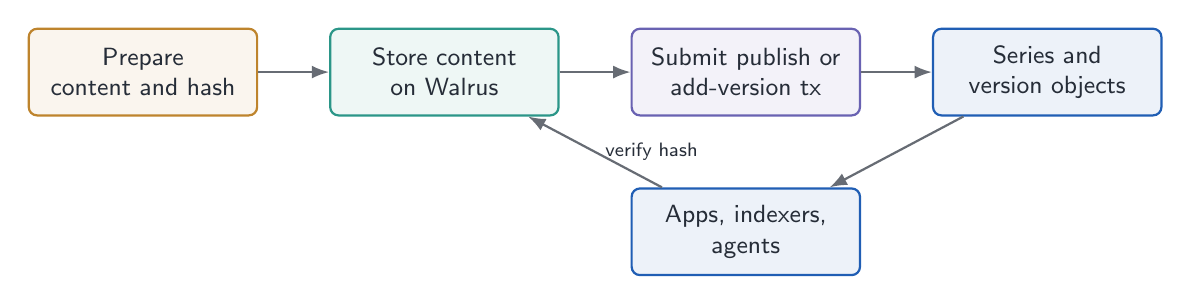
\begin{tikzpicture}[node distance=9mm]
  \node[step=gold] (prepare) {Prepare\\content and hash};
  \node[step=green, right=of prepare] (walrus) {Store content\\on Walrus};
  \node[step=purple, right=of walrus] (version) {Submit publish or\\add-version tx};
  \node[step=blue, right=of version] (series) {Series and\\version objects};
  \node[step=blue, below=of version] (clients) {Apps, indexers,\\agents};
  \draw[arrow] (prepare) -- (walrus);
  \draw[arrow] (walrus) -- (version);
  \draw[arrow] (version) -- (series);
  \draw[arrow] (series) -- (clients);
  \draw[arrow] (clients) -- node[right, font=\sffamily\scriptsize, text=textgray] {verify hash} (walrus);
\end{tikzpicture}
\end{document}
